\newpage
\section{Visionneuse Openseadragon}
\label{sec:seadragon}
OpenSeadragon est une visionneuse d’image haute résolution, modulable et open source. De plus, elle est adaptée aux périphériques pc et mobile, ce qui convient à notre projet. Nous utiliserons la version 2.1.0. OpenSeadragon est un plugin implémenté en Javascript. La visionneuse sera insérée dans la page HTML de consultation de documents à travers un script comme l'illustre la figure \ref{seadragon}. 

Pour notre projet nous allons utiliser les fonctionnalités d'OpenSeadragon suivantes : 
\begin{itemize}
	\item l'affichage de l'image associée au document : Opensedragon prend en charge plusieurs formats d'image. Dans notre cas, les images de presse ancienne étant très grandes, l'utilisation d'un format d'image simple (JPG,PNG,...) rend la visionneuse moins performantes. Nous allons donc utiliser un outils : PHP Deep Zoom Tools qui permet d'avoir des images tuilées au format .dzi (Deep Zoom Image), beaucoup plus performantes avec OpenSeadragon.
	\item les boutons de zoom/dézoom 
	\item les boutons de navigation, rotation
	\item les calques : utiles pour délimiter les articles, ou rajouter des tags par exemple. Dans notre cas, nous rajouterons à Openseadragon le plugin (Javascript également) SVG-overlay qui permet de réaliser ces calques.
	\end{itemize}
	
	  \begin{figure}[H]
        \centering
        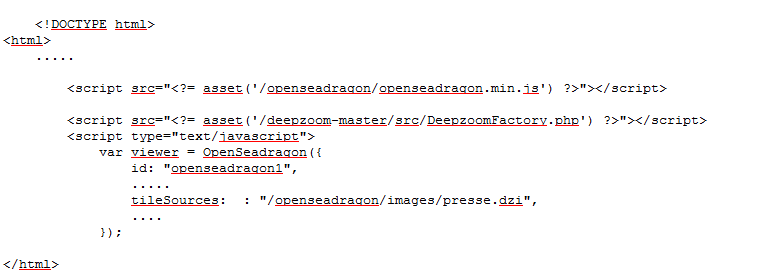
\includegraphics[width=\textwidth]{figure/osd.png}
            \caption{Architecture globale de la plateforme}
            \label{seadragon}
    \end{figure}
	
	





